\section{Auswertung}
\subsection{Messung des Kontrasts der Apparatur}
Für die Ermittlung des Kontrasts des Interferometer wird ein Laser mit einer Wellenlänge von $\lambda_{vac}=\SI{623.99}{\nano\meter}$ verwendet.
Aus den gemessenen Intensitäten wird dann mithilfe von Formel \eqref{eq:kontrast} der Kontrast berechnet.
Die Messwerte, sowie der berechnete Kontrast sind in Tabelle \ref{tab:Kontrast} zusammengestellt.
Das Maximum des Kontrasts liegt bei einem Winkel von 60\circ.\\
\begin{figure}[H]
  \center
  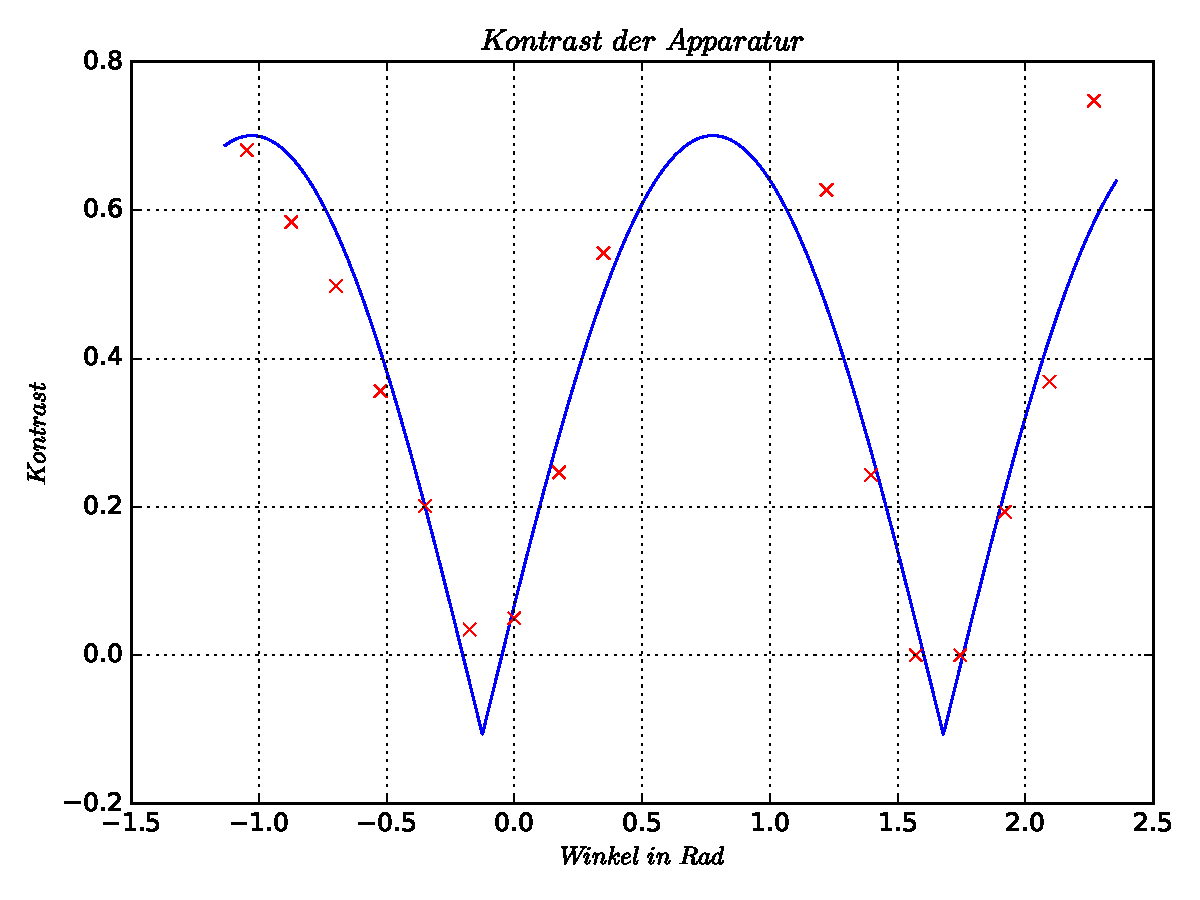
\includegraphics[width=0.65\textwidth]{./plots/kontrastplot.pdf}
  \caption{Winkel der Platten und aus den gemessenen Intensitäten errechneter Kontrast.}
  \label{fig:kontrastplot}
\end{figure}
\begin{table}[H]
  \center
  \caption{Zu unterschiedlichen Winkeln gemessene Intensitäten dazu errechneter Kontrast.}
  \label{tab:Kontrast}
\begin{tabular}{c|c|c|c}
  Winkel in Grad& $U_{min}$ in mV& $U_{max}$ in mV& Kontrast\\
  \hline
  -60 &    -1085&       25& 0.6808\\
  -50 &     -975&       25& 0.5841\\
  -40 &  -969.75&   -37.50& 0.4979\\
  -30 &  -969.75&  -281.25& 0.3561\\
  -20 & -1118.75& -1012.50& 0.2013\\
  -10 & -1106.75&  -668.75& 0.0347\\
  0   & -1118.75& -1043.75& 0.0498\\
  10  & -1118.75&  -743.75& 0.2465\\
  20  & -1118.75&  -531.25& 0.5422\\
  30  & -1118.75&  -375.00& 0.9255\\
  40  & -1118.75&  -293.75& 0.95\\
  45  & -1118.75&  -212.50& 0.955\\
  50  & -1118.75&   -87.50& 0.8549\\
  \hline
  60  & -1118.75&   -18.75& 0.9670\\
  \hline
  70  & -1118.75&  -256.25& 0.6273\\
  80  & -1118.75&  -681.25& 0.2431\\
  90  &        -&        -&      0\\
  100 &        -&        -&      0\\
  110 & -1118.75&  -756.25& 0.1933\\
  120 &  -1125.0&  -518.75& 0.3688\\
  130 &  -1125.0&  -162.50& 0.7476\\
\end{tabular}
\end{table}
In \ref{fig:kontrastplot} ist der Kontrast in Abhängigkeit des Drehwinkels der Platten aufgetragen und mithilfe von $curve-fit$ gefitted worden.
Um die Messwerte optimal durch einen Fit zu approximieren wurden die Messwerte zwischen $30^\circ$ und $60^\circ$ aus dem Diagramm entfernt. Bei $90^\circ$ und $100^\circ$ sind beide Intensitäten im Hintergrundrauschen untergegangen, woraus sich der Kontrast von 0 ergibt.\\
\subsection{Berechnung des Brechungsindex der Platten}
  In der Anleitung \cite{Anleitung} finden sich zur Berechnung des Brechungsindex der Platten folgende Herstellerangaben:\\
\begin{center}
  $T = \SI{1}{\milli\meter}$, $n_{\symup{Lit}}=1.35$, $\delta =10$\circ
\end{center}
Anhand dieser Angaben, sowie den gemessenen Werten, wird mithilfe von Formel \eqref{eq:index} aus der Theorie der Brechungsindex der Platten errechnet.
Die berechneten Werte sind in Tabelle \ref{tab:plattenindex} einzusehen.\\
\begin{table}[H]
  \center
  \caption{Gemessene Counts bei einer Drehung der Platten um ca. $\theta=10^\circ$ und Mittelwert des berechneten Brechungsindex.}
	\label{tab:plattenindex}
  \begin{tabular}{c|c|c|c}
    Messung& Counts M& Brechungsindex n& Fehler\\
    \hline
    1& 55& 1.049& 0.036\\
    2& 40& 1.038& 0.027\\
    3& 55& 0.750& 1.159\\%Bullshit messung! in den messwerten ist auch n fetter sprung.
    4& 51& 1.015& 0.050\\
    5& 55& 1.015& 0.054\\
    6& 43& 1.036& 0.031\\
    7& 37& 1.023& 0.023\\
    8& 34& 1.034& 0.023\\
  \end{tabular}
\end{table}
\subsection{Berechnung des Brechungsindex von Luft}
In den Tabellen \ref{tab:druckdaten1} und \ref{tab:druckdaten2} sind die mithilfe von Formel \eqref{eq:luft} berechneten Werte des Brechungsindex von Luft bei steigendem Druck zu sehen.
Die Wellenlänge des Lasers beträgt nach wie vor $\lambda_{vac}=\SI{632.99}{\nano\meter}$. Die Länge der Gaszelle ist durch $L=\SI{10}{\centi\meter}$ gegeben.
\begin{table}[H]
  \center
  \caption{Brechungsindex von Luft bei steigendem Druck in 100 mbar Schritten.}
  \label{tab:druckdaten1}
 \begin{tabular}{c|c|c|c}
   $p_1$ in mbar&$n_1$ &$p_2$ in mbar &$n_2$\\
   \hline
   11  &1.000 070 & 12  & 1.000 076\\
   100 &1.000 633 & 100 & 1.000 633\\
   200 &1.001 266 & 200 & 1.001 266\\
   300 &1.001 899 & 300 & 1.001 899\\
   400 &1.002 532 & 400 & 1.002 532\\
   500 &1.003 165 & 500 & 1.003 165\\
   600 &1.003 798 & 600 & 1.003 798\\
   700 &1.004 431 & 700 & 1.004 431\\
   800 &1.005 064 & 800 & 1.005 064\\
   900 &1.005 697 & 900 & 1.005 697\\
   995 &1.006 298 & 995 & 1.006 298\\
 \end{tabular}
\end{table}
\begin{table}[H]
    \center
    \caption{Brechungsindex von Luft bei steigendem Druck in 50 mbar Schritten.}
    \label{tab:druckdaten2}
    \begin{tabular}{c|c|c|c}
      $p_3$ in mbar&$n_3$ &$p_4$ in mbar &$n_4$\\
      \hline
      8  & 1.000 051& 8  & 1.000 051\\
      50 & 1.000 317& 50 & 1.000 317\\
      100& 1.000 633& 100& 1.000 633\\
      150& 1.000 949& 150& 1.000 949\\
      200& 1.001 266& 200& 1.001 266\\
      250& 1.001 582& 250& 1.001 582\\
      300& 1.001 899& 300& 1.001 899\\
      350& 1.002 215& 350& 1.002 215\\
      400& 1.002 532& 400& 1.002 320\\
      450& 1.002 848& 450& 1.002 848\\
      500& 1.003 165& 500& 1.003 165\\
      550& 1.003 481& 550& 1.003 481\\
      600& 1.003 798& 600& 1.003 798\\
      650& 1.004 114& 650& 1.004 114\\
      700& 1.004 431& 700& 1.004 431\\
      750& 1.004 747& 750& 1.004 747\\
      800& 1.005 064& 800& 1.005 064\\
      850& 1.005 380& 850& 1.005 380\\
      900& 1.005 697& 900& 1.005 697\\
      950& 1.006 013& 950& 1.006 013\\
      995& 1.006 298& 995& 1.006 298\\
    \end{tabular}
\end{table}


